\documentclass[10pt, compress]{beamer}

\usetheme{metropolis}           % Use metropolis theme

\usepackage{natbib}
\bibliographystyle{unsrt}
\usepackage{booktabs}
\usepackage[scale=2]{ccicons}
\usefonttheme[onlymath]{serif}

%\usemintedstyle{trac}

\title{A review on methods for Bayesian hierarchical clustering}
\subtitle{}
\date{\today}
\author{Sharad Vikram}
\institute{UCSD}

\begin{document}

\maketitle

\section{Background}

\begin{frame}{Unsupervised learning}
  In unsupervised learning, we are interested in finding
        underlying structure
        in data.

  Current methods include:
  \begin{itemize}
    \item<2-> \textbf{Dimensionality reduction:} finding low-dimensional
      representations of high-dimensional data
    \item<3-> \textbf{Clustering:} discovering natural groups
      in data
  \end{itemize}
\end{frame}

\begin{frame}{Clustering}
  The most popular methods for clustering produce
  flat clusterings.

  A \alert{flat clustering} is a partition of a set of data,
  or an assignment of each data point into one of
  several disjoint sets.

  \begin{align}
    \{1, 2, \ldots, N\} \rightarrow \{\{1,2\}, \{3, 4, 5\}, \ldots, \{N - 1, N\}\}
  \end{align}
\end{frame}

\begin{frame}{Flat clustering}
  The most popular algorithm for flat clustering is \alert{k-means}.
  \begin{enumerate}
    \item<2-> Pick a number of clusters $K$.
    \item<3-> Randomly initialize cluster centers $\{\mu_1, \ldots, \mu_K\}$.
    \item<4-> Alternate until convergence:
      \begin{itemize}
        \item Assign each data point to its closest cluster center.
        \item Assign each cluster center to the mean of its assigned data points.
      \end{itemize}
  \end{enumerate}
  This is equivalent to optimizing the loss function:
  \begin{align}
    L(\mu_1, \ldots, \mu_K) = \sum_{i = 1}^N \min_k \|x_i - \mu_k\|^2_2
  \end{align}
\end{frame}

\begin{frame}{Flat clustering: pros and cons}
  \begin{table}
    \begin{tabular}{lr}
      \toprule
      Pros & Cons \\
      \midrule
      Simple algorithms &  Requires specification of $k$ (in general)\\
      Efficient algorithms & \\
      Theoretical understanding & \\
      \bottomrule
    \end{tabular}
  \end{table}
\end{frame}

\begin{frame}{Hierarchical clustering}
  In \alert{hierarchical clustering}, data
  is recursively partitioned to form a tree (typically binary),
  also called a hierarchy.

  %TODO: insert image

  Each leaf in the tree is a single data point,
  The root is the grouping of all data points
  into a single cluster and internal nodes
  are groupings of different granularities.
\end{frame}

\begin{frame}{Traditional hierarchical clustering algorithms}
  Hierarchical clustering algorithms can be broadly broken
  down into two categories:

  \begin{itemize}
    \item<2-> \textbf{Agglomerative (bottom-up):} the tree is built by
      beginning with just singleton clusters (leaves) and
      iteratively merging them until we have one cluster (root)
    \item<3-> \textbf{Divisive (top-down):} the tree is built
      by beginning with a single cluster (root) and
      recursively partitioning it until we
      have just singleton clusters (leaves)
  \end{itemize}
\end{frame}

\begin{frame}{Agglomerative clustering}
  The inputs to an agglomerative clustering algorithm
  are:
  \begin{itemize}
    \item<2-> Dataset $X = \{x_i\}_{i = 1}^N$
    \item<3-> Dissimilarity function $d(x, x')$
    \item<4-> Linkage criterion $D(A, B)$.
  \end{itemize}

\end{frame}

\begin{frame}{Dissimilarity functions}

  A dissimilarity function measures how
  different two data points are from each other.

  Example dissimilarity functions include:
  \begin{itemize}
    \item Euclidean distance: $d(x, x') = \|x - x'\|_2^2$
    \item Manhattan distance: $d(x, x') = \|x - x'\|_1$
    \item Mahalanobis distance: $d(x, x') = (x - x')^T\Sigma(x - x')$
  \end{itemize}
\end{frame}

\begin{frame}{Linkage criteria}

  A linkage measures how
  different two \textbf{clusters} are from each other
  in terms of dissimilarity function $d$.

  Example linkage criteria include:
  \begin{itemize}
    \item<2-> Single linkage: $D(A, B) = \min_{i \in A, j\in B} d(x_i, x_j)$
    \item<3-> Complete linkage: $D(A, B) = \max_{i \in A, j\in B} d(x_i, x_j)$
    \item<4-> Average linkage: $D(A, B) = \frac{1}{|A||B|}\sum_{i \in A, j\in B} d(x_i, x_j)$
  \end{itemize}
\end{frame}

\begin{frame}{Agglomerative clustering examples}
  \begin{figure}
    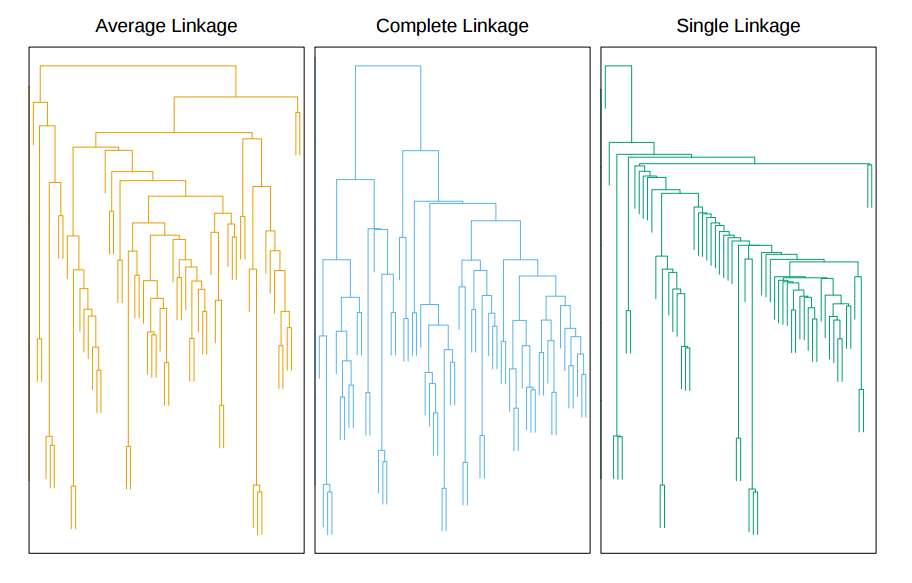
\includegraphics[width=\textwidth]{img/dendrograms}
    \caption{Trees produced by agglomerative clustering algorithms
    with different linkage criteria. Source: \citep{Hastie2009}}
    \label{fig:dendrograms}
  \end{figure}
\end{frame}

\begin{frame}{Divisive clustering}
  In divisive clustering, we begin with the root cluster
  and recursively partition it until we are left with
  singleton leaf clusters.
\end{frame}

\begin{frame}{Ambiguous data}
  Consider the following scenarios when the hierarchy is
  \textbf{ambiguous}.

  The aforementioned methods produce a single tree,
  but we need a more flexible framework to handle
  this scenario.
\end{frame}

\begin{frame}{Probabilistic reasoning}
  A more general approach is to
  model our uncertainty with \textbf{probability}.

  Instead of outputting a single tree,
  we output a probability distribution over all possible
  trees.
\end{frame}

\begin{frame}{Bayesian learning}
  We take a quick detour to review Bayesian learning.
\end{frame}

\begin{frame}{References}
  \bibliography{main}
\end{frame}

\begin{frame}[fragile]
  \frametitle{mtheme}

  The \emph{mtheme} is a Beamer theme with minimal visual noise inspired by the
  \href{https://github.com/hsrmbeamertheme/hsrmbeamertheme}{\textsc{hsrm} Beamer
  Theme} by Benjamin Weiss.

  Enable the theme by loading

  %\begin{minted}[fontsize=\small]{latex}
    %\documentclass{beamer}
    %\usetheme{m}
  %\end{minted}

  Note, that you have to have Mozilla's \emph{Fira Sans} font and XeTeX
  installed to enjoy this wonderful typography.
\end{frame}

\begin{frame}[fragile]
  \frametitle{Sections}
  Sections group slides of the same topic

  %\begin{minted}[fontsize=\small]{latex}
    %\section{Elements}
  %\end{minted}

  for which the \emph{mtheme} provides a nice progress indicator \ldots
\end{frame}

\section{Elements}

\begin{frame}[fragile]
  \frametitle{Typography}
      %\begin{minted}[fontsize=\small]{latex}
%The theme provides sensible defaults to \emph{emphasis}
%text, \alert{accent} parts or show \textbf{bold} results.
      %\end{minted}

  \begin{center}becomes\end{center}

  The theme provides sensible defaults to \emph{emphasis} text,
  \alert{accent} parts or show \textbf{bold} results.
\end{frame}
\begin{frame}{Lists}
  \begin{columns}[onlytextwidth]
    \column{0.5\textwidth}
      Items
      \begin{itemize}
        \item Milk \item Eggs \item Potatos
      \end{itemize}

    \column{0.5\textwidth}
      Enumerations
      \begin{enumerate}
        \item First, \item Second and \item Last.
      \end{enumerate}
  \end{columns}
\end{frame}
\begin{frame}{Descriptions}
  \begin{description}
    \item[PowerPoint] Meeh.
    \item[Beamer] Yeeeha.
  \end{description}
\end{frame}
\begin{frame}{Animation}
  \begin{itemize}[<+- | alert@+>]
    \item \alert<4>{This is\only<4>{ really} important}
    \item Now this
    \item And now this
  \end{itemize}
\end{frame}
\begin{frame}{Figures}
  \begin{figure}
    \caption{Rotated square from
    \href{http://www.texample.net/tikz/examples/rotated-polygons/}{texample.net}.}
  \end{figure}
\end{frame}
\begin{frame}{Tables}
  \begin{table}
    \caption{Largest cities in the world (source: Wikipedia)}
    \begin{tabular}{lr}
      \toprule
      City & Population\\
      \midrule
      Mexico City & 20,116,842\\
      Shanghai & 19,210,000\\
      Peking & 15,796,450\\
      Istanbul & 14,160,467\\
      \bottomrule
    \end{tabular}
  \end{table}
\end{frame}
\begin{frame}{Blocks}

  \begin{block}{This is a block title}
    This is soothing.
  \end{block}

\end{frame}
\begin{frame}{Math}
  \begin{equation*}
    e = \lim_{n\to \infty} \left(1 + \frac{1}{n}\right)^n
  \end{equation*}
\end{frame}
\begin{frame}{Quotes}
  \begin{quote}
    Veni, Vidi, Vici
  \end{quote}
\end{frame}

%\plain{Dark background}{\vspace{-2em}\begin{center}\includegraphics[width=\textwidth]{images/valley.jpg}\end{center}}

\section{Conclusion}

\begin{frame}{Summary}

  Get the source of this theme and the demo presentation from

  \begin{center}\url{github.com/matze/mtheme}\end{center}

  The theme \emph{itself} is licensed under a
  \href{http://creativecommons.org/licenses/by-sa/4.0/}{Creative Commons
  Attribution-ShareAlike 4.0 International License}.

  \begin{center}\ccbysa\end{center}

\end{frame}

\plain{}{Questions?}

\end{document}
